\documentclass[twoside,11pt]{article}

% Any additional packages needed should be included after jmlr2e.
% Note that jmlr2e.sty includes epsfig, amssymb, natbib and graphicx,
% and defines many common macros, such as 'proof' and 'example'.
%
% It also sets the bibliographystyle to plainnat; for more information on
% natbib citation styles, see the natbib documentation, a copy of which
% is archived at http://www.jmlr.org/format/natbib.pdf

\usepackage{jmlr2e}
\usepackage{algorithm}
\usepackage{natbib}
\usepackage{amsmath}
\usepackage{float}
\usepackage{subcaption}
\usepackage{hyperref}


% Definitions of handy macros can go here

\newcommand{\dataset}{{\cal D}}
\newcommand{\fracpartial}[2]{\frac{\partial #1}{\partial  #2}}

% Heading arguments are {volume}{year}{pages}{submitted}{published}{author-full-names}

\jmlrheading{19}{2018}{1-8}{12/00}{13/00}{Jia Guo, Masaya Tsukamoto, Zihan Wang and Guangting Yu}

% Short headings should be running head and authors last names

\ShortHeadings{Spectral Clustering}{Guo, Tsukamoto, Wang and Yu}
\firstpageno{1}

\begin{document}

\title{Spectral Clustering}

\author{\name Jia Guo \email guojia@umich.edu \\
        \addr Department of Mathematics\\
        University of Michigan\\
        Ann Arbor, MI 48109, USA
        \AND
        \name Masaya Tsukamoto \email masayats@umich.edu \\
        \addr Department of Mathematics\\
        University of Michigan\\
        Ann Arbor, MI 48109, USA
        \AND
        \name Zihan Wang \email wzihan@umich.edu \\
        \addr Department of Climate and Space Sciences and Engineering\\
        University of Michigan\\
        Ann Arbor, MI 48109, USA
        \AND
        \name Guangting Yu \email yugtmath@umich.edu \\
        \addr Department of Mathematics\\
        University of Michigan\\
        Ann Arbor, MI 48109, USA}

\editor{Aniket,}

\maketitle

\begin{abstract}
We study a spectral clustering method based on local principal component analysis (PCA).
Instead of dealing with pair-wise distances between points like the previous algorithms do, this algorithm is able to resolve intersections.
Especially, the new setting requires the surfaces to be smooth.
Within this smoothness assumption, there is a mathematical theorem supporting the new algorithms.
Furthermore, we apply this algorithm to autograding arithmetic problems.
\end{abstract}

\begin{keywords}
Spectral Clustering, Local principal component analysis, Autograding
\end{keywords}

%!TEX root = main.tex

% \documentclass[11pt, oneside]{article}   	% use "amsart" instead of "article" for AMSLaTeX format
% \usepackage{geometry}                		% See geometry.pdf to learn the layout options. There are lots.
% \geometry{letterpaper}                   		% ... or a4paper or a5paper or ... 
% \usepackage{graphicx}				% Use pdf, png, jpg, or eps with pdflatex; use eps in DVI mode
% 								% TeX will automatically convert eps --> pdf in pdflatex		
% \usepackage{amssymb}
% \usepackage{natbib}
% \usepackage{amsmath}

% \usepackage{algorithm} % for algorithm
% \usepackage{amsfonts} % for \mathbb{R}

% \begin{document}


\section{Introduction}


The recognition of handwritten digit strings is relevant in a variety of applications in our daily life.
In post office, handwritten ZIP code can be recognized automatically.
At primary school, the grading of arithmetic problems can be completed in one second with a smart phone application.
However, there are still several challenges in this field.
One bottleneck is related with the segmentation module, which segments a string of characters into individual one.
The reason behind is that strings sometimes are not neatly written, e.g. overlapping, touching, and intersecting (\autoref{example}).
Many algorithms have been proposed to deal with this problem.
They can mainly be divided into two categories \citep{casey1996}.
The first one is segmentation-recognition, which means segmentation is completed before recognition.
The second one is recognition based, where the algorithm yields a list of segmentation hypotheses and then assesses each of them through the recognition process.
This method will take the information of the foreground and background into account.
Recently, segmentation-free methods are also introduced \citep{hochuli2018}.

\begin{figure}[ht] %  figure placement: here, top, bottom, or page
   \centering
   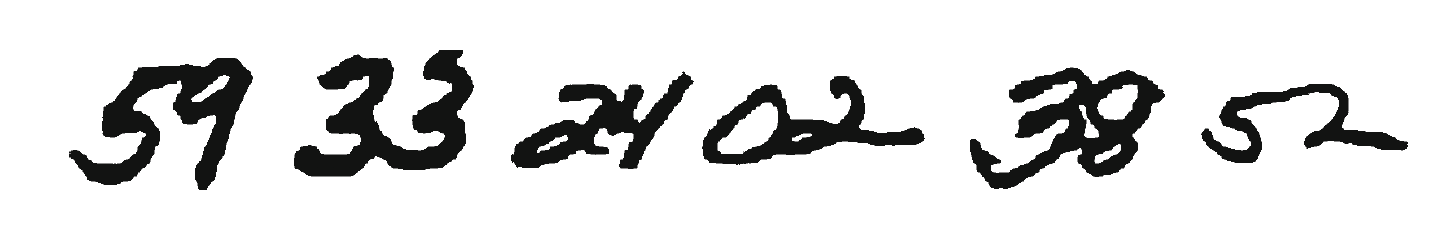
\includegraphics[width=2in]{example.png} 
   \caption{Variability of connections between handwritten digits.}
   \label{example}
\end{figure}

In this project, the main goal is to deal with the intersections in the handwritten digit strings.
Here we will focus on segmentation-recognition implementing the spectral clustering based on local principle component analysis (PCA) \citep{arias2017}.
A straightforward idea for segmentation is to utilize spectral clustering \citep{ng2002}.
However, a fatal drawback of spectral clustering is that it cannot separate two intersecting clusters.
Thus, it cannot deal with the segmentation in handwritten digits.
\citet{shashua2006} claim that a multiway affinity is needed to capture complex structure in data (e.g. intersection) beyond proximity attributes.
\citet{fan2006} first implemented subspace clustering based on local PCA.
Later, \citet{goldberg2009} developed a spectral clustering method within a semi-supervised learning framework.
Continuing this line of work, \citep{arias2011} suggest a spectral clustering method based on the estimation of the local linear structure (tangent bundle) via local PCA.
There are also two concurrent publications \citep{wang2011, gong2012} with quite similar methods.

The rest of the report is organized as follows.
In Section 2, we will show authors' algorithms to implement spectral clustering based on local PCA.
The rationale behind the algorithm will be briefly discussed.
In Section 3, we will analyze the results of the algorithm.
In Section 4, we will show one application of this algorithm.
In Section 5, we will present the conclusion.

\section{Methodology}
% \makeatletter
% \renewcommand{\thealgorithm}{} % remove Algorithm number such as Algorithm "4"
% \makeatother
% \begin{algorithm}[htbp]
% \caption{Spectral Clustering Based on Local PCA}

There are four different algorithms on spectral clustering provided in the paper \citep{arias2017}.
Algorithm 1 gives the sketch of the standard spectral graph partitioning with given affinity matrix \(W\).
Different variants, Algorithm 2 and 3 are also proposed.
One of the biggest defference is the affinity matrix 
$W_{ij} = \boldsymbol{1}_{ \{ || \boldsymbol{y}_i - \boldsymbol{y}_j || \leq \epsilon \} } 
 \boldsymbol{1}_{ \{ || \boldsymbol{C}_i - \boldsymbol{C}_j || \leq \eta r^2 \}}  $ in Algorithm 2 and 
$W_{ij} = \boldsymbol{1}_{ \{ || \boldsymbol{y}_i - \boldsymbol{y}_j || \leq \epsilon \} } 
 \boldsymbol{1}_{ \{ || \boldsymbol{Q}_i - \boldsymbol{Q}_j || \leq \eta \}}  $ in Algorithm 3. 
They are kinds of ``hard" versions and more tractable, where Theorem 1 introduced below holds.
However, the author found  Algorithm 4 performs better via numerical experiments.
So we just provide Algorithm 4 below.

\noindent\hrulefill\\
\textbf{Input:} \newline
Data points $\boldsymbol{x}_1, ..., \boldsymbol{x}_n \in \mathbb{R}^D$; neighborhood radius $r>0$; spatial scale $\epsilon>0$; projection scale $\eta>0$; intrinsic dimension $d$; number of clusters $K$. \vspace{0.1in} \newline
\textbf{Steps:  (called ``Algorithm 4" in the paper)}
\begin{enumerate}
\item Pick one point $\boldsymbol{y}_1$ at random from the data.
Pick another point $\boldsymbol{y}_2$ among the data points not included in neighborhood $N_r(\boldsymbol{y}_1)$, and repeat the process, selecting centers $\boldsymbol{y}_1$, ..., $\boldsymbol{y}_{n_0}$.
Here we define the neighborhood $N_r(\boldsymbol{x})=\{\boldsymbol{x}_j : ||\boldsymbol{x}-\boldsymbol{x}_j|| \leqslant r\}$ for any point $\boldsymbol{x} \in \mathbb{R}^D$ and $r>0$, given a data set $\boldsymbol{x}_1, ..., \boldsymbol{x}_n$.
\item For each $i$ = 1, ..., $n_0$, compute the sample covariance matrix $\boldsymbol{C}_i$ of $N_r(\boldsymbol{y}_i)$.
Let $\boldsymbol{Q}_i$ denote the orthogonal projection onto the space spanned by the top $d$ eigenvectors of $\boldsymbol{C}_i$.
\item Compute the following affinities between center pairs:
\begin{equation}
W_{ij}=\exp \left( -\frac{||\boldsymbol{y}_i-\boldsymbol{y}_j||^2}{\epsilon^2} \right) \cdot \exp \left(-\frac{||\boldsymbol{Q}_i-\boldsymbol{Q}_j||^2}{\eta^2} \right)
\end{equation}
\item (Spectral Graph Partitioning) Compute $\boldsymbol{Z} = (Z_{ij})$ according to $Z_{ij} = W_{ij}/\sqrt{\Delta_i \Delta_j}$, with $\Delta_i=\Sigma_{j=1}^{n} W_{ij}$.
Extract the top $K$ eigenvectors of $Z$.
Renormalize each row of the resulting $n \times K$ matrix.
Apply $K$-means to the row vectors.
\item The data points are clustered according to the closest center in Euclidean distance.
\end{enumerate}
\noindent\hrulefill\\
% \end{algorithm}

The main idea is that we first divide the original data points into small circles (or spheres) $N(\boldsymbol{y}_i)$ with the radius $r$.
Then we grab the information about the direction of the local data arrangement in each circle through the sample covariance matrix $\boldsymbol{C}_i$ and extract the information as the projection matrix $\boldsymbol{Q}_i$.
The affinities $W_{ij}$ are set so that circles are classified as the same cluster if they are geometrically close and the local directions of the data arrangement are similar.



\autoref{cross} is the simplest example of the clustering by this algorithm ($K = 2$, $r = 15.0$, $\epsilon = 15.0$, $\eta = 0.5$).
The cross-shaped data is seccessfully separated by the intersection.

\begin{figure}[htbp]
\centering
\vspace{-1em}
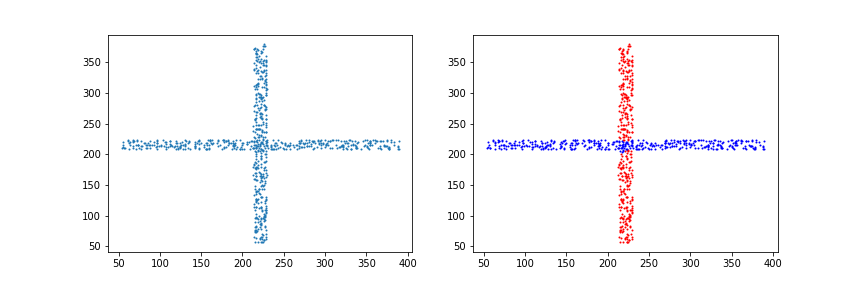
\includegraphics[width=0.8  \textwidth]{cross_shaped.png}
\vspace{-1em}
\caption{Clustering example}
\label{cross}
\end{figure}


% \end{document}  


\section{Theoretical Analysis and Examples}
While the analysis of Algorithm 4 seems within reach, there are some complications due to the fact that points near the intersection may form a cluster of their own.
See \autoref{fig1}.
The vertical line and $\infty$-shaped line are sccessfully separated by Algorithm 4 ($K = 2$, $r = 15.0$, $\epsilon = 15.0$, $\eta = 0.3$).
But points near the intersectionis are fully classified as ``Blue" group. 
\begin{figure}[htbp]
\centering
\vspace{-1em}
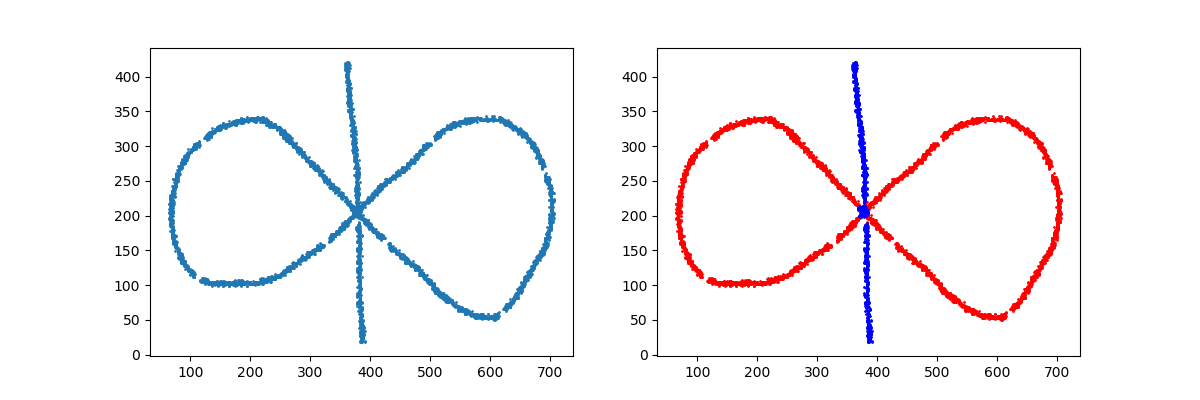
\includegraphics[width=0.9  \textwidth]{infinity_shape.png}
\vspace{-1em}
\caption{Example of intersection cluster}
\label{fig1}
\end{figure}

Instead, the authors mainly focus on some simpler variants described in Algorithm 2 and Algorithm 3, and then give a comment on the analysis of Algorithm 4.
More theoretical results on intersecting manifolds 
refer to \cite{arias2011},\cite{chen2009},\cite{soltanolkotabi2012}.
The generative model is a natural mathematical framework for multi-manifold learning where points are sampled in the vicinity of smooth surfaces embedded in Euclidean space.
One can see in the numerical experiments that the Algorithm 4 fails to deal with phenomenon that the intersection with a sharp corner.
See \autoref{sharp_720}. This is obtained by  Algorithm 4  ($K = 3$, $r = 10.0$, $\epsilon = 10.0$, $\eta = 0.5$), and is a typical result of this algorithm, where ``2" is separated by the bottomleft sharp corner.
\begin{figure}[htbp]
\centering
\vspace{-1em}
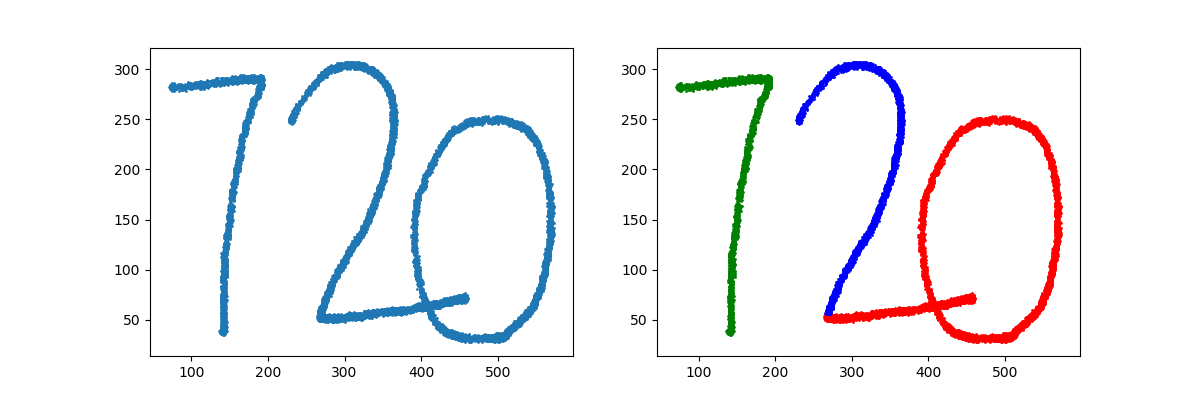
\includegraphics[width=0.9  \textwidth]{sharp_720.png}
\vspace{-1em}
\caption{Failure at the corner}
\label{sharp_720}
\end{figure}

To clarify the characteristics of the algorithm, additional ``720"-shaped data which were written intentionally smoothly are applied below.  See figure \autoref{smooth_720}, where both of the above and below are obtained by Algorithm 4 with the same parameters $K = 3$, $r = 10.0$, $\epsilon = 10.0$, $\eta = 0.5$.
Due to smoothness, ``720" are successfully separated into 3 digits in both figures.

%\begin{figure}[htbp]
%\hspace{-3em}
%\subfigure{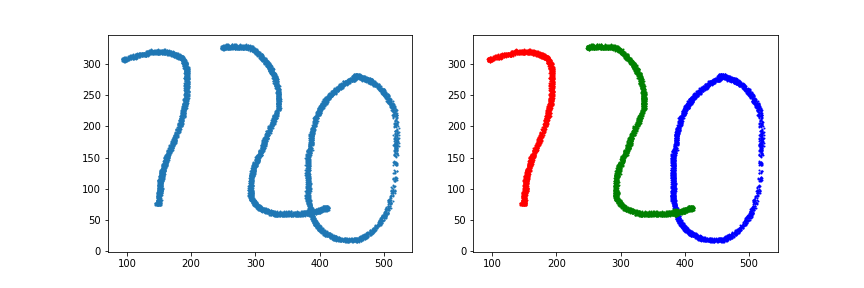
\includegraphics[width=0.6  \textwidth]{smooth_720_1.png}}
%\hspace{-2em}
%\subfigure{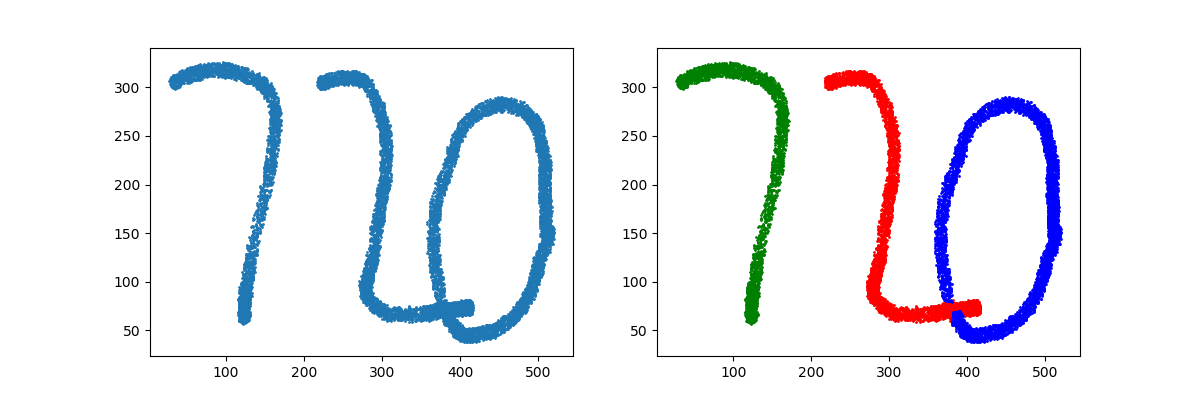
\includegraphics[width=0.6  \textwidth]{smooth_720_2.png}}
%\caption{Successful results with smooth data}
%\label{smooth_720}
%\end{figure}
\begin{figure}[htbp]
\centering
\vspace{-1em}
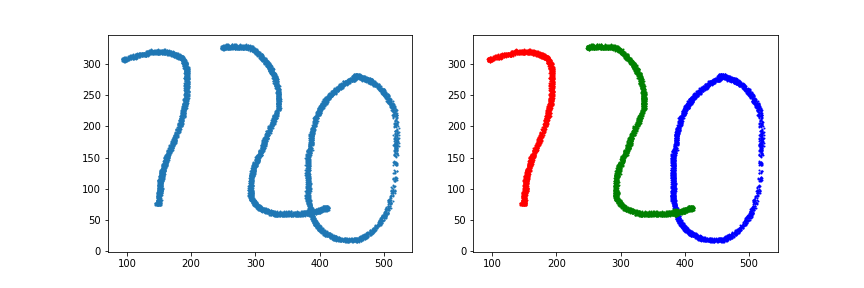
\includegraphics[width=0.8  \textwidth]{smooth_720_1.png}
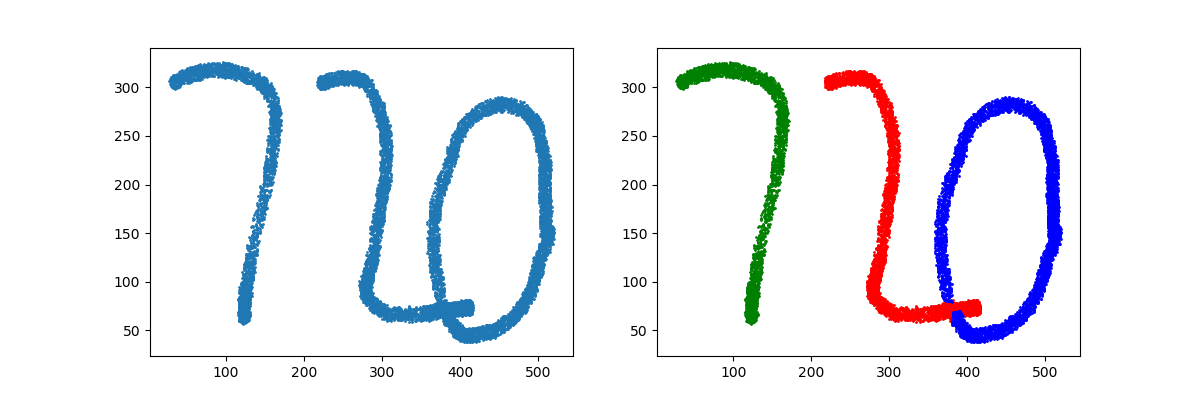
\includegraphics[width=0.8  \textwidth]{smooth_720_2.png}
\vspace{-1em}
\caption{Successful results with smooth data}
\label{smooth_720}
\end{figure}

Precisely, $K=2$ and each surface is a connected, $C^2$ and compact submanifold without boundary and of dimension $d$ embedded in $\mathbb R^D$.
Any such surface has a positive reach, which is what we use to quantify smoothness.
The clusters are generated as follows.
Each data point $x_i$ is drawn according to
$$ x_i = s_i + z_i $$
where $s_i$ is from the uniform distribution over
$S_1\cup S_2$ and $z_i$
is an additive noise term satisfying $||z_i||\le \tau$.
The main theorem of the paper is given below.
\begin{theorem}
Consider two connected, compact, twice continuously differentiable submanifolds
without boundary, of same dimension \(d\), intersecting at a strictly positive angle, with the intersection set having strictly positive reach.
Assume the parameters are set so that
$$
\tau\le \frac{r\eta}{C},\ \ r\le\frac{\epsilon}{C},\ \ \epsilon\le\frac{\eta}{C},\ \ \eta\le\frac{1}{C}
$$
for large constant $C\ge 1$.
Then with probability at least $1-Cn\exp(- nr^d\eta^2/C)$:
\begin{itemize}
\item Algorithm 2 returns exactly two groups such that two points from different clusters are not grouped together unless one of them is within distance \(C_r\) from the intersection.
\item Algorithm 3 returns at least two groups, and such that two points from different clusters are not grouped together unless one of them is within distance \(C_r\) from the intersection.
\end{itemize}
\end{theorem}

\begin{proof}
We give a sketch of proof of algorithm 2 and refers to the paper for more details. Some important notation:
$$
I^*=\{i: K_j=K_i,\ \forall j\in\Xi_i  \},\ \ \ \Xi_i=\{j\ne i, s_j\in N_r(s_i)   \}
$$
Thus $I^*$ indexes the points whose neighborhoods do not contain points from the other cluster.
\begin{enumerate}
\item Assume $\tau=0$, and then explain for how things change for $\tau>0$. Deriving a concentration inequality for local covariances with large constant $C$.
\item Then show that among points away from the intersection, those that are in the same cluster are neighbors in the graph if they are within distance $\epsilon$, while those in different clusters cannot be neighbors in the graph.
\item Confirming that step 2 in algorithm 2 can eliminate all points which are not included in $I^*$, and  the points removed are within distance $Cr$ of the intersection, furthermore,  points removed are within distance $Cr$ of the intersection.
\item Concluding that in step 4, algorithm 2 returns two graphs, and each group covers an entire cluster except for points within distance $O(r)$ of the intersection.
\end{enumerate}
\end{proof}

To conclude, the key point of the approach is using principal component analysis to study the local behavior of data, and then use the information about affinity to generate a new local neighborhood graph.
However, the selection of the parameters is quite sensitive to the final output, it is still a quite acceptable approach in many applications and perform well in particular example.

For comparison, results with different parameters are described in \autoref{fig4}, \autoref{fig5}, and \autoref{fig6}. If not explicitly mentioned, parameters $K = 3$, $r = 10.0$, $\epsilon = 10.0$, $\eta = 0.5$ are used.

\begin{figure}[htbp]
\centering
\hspace{-2em}
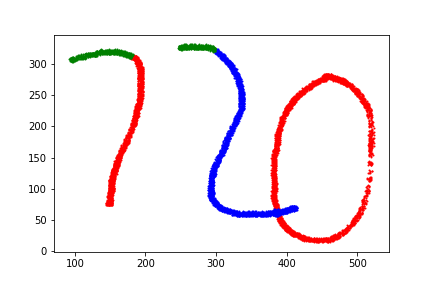
\includegraphics[width=0.37  \textwidth]{eta_small.png}
\hspace{-2em}
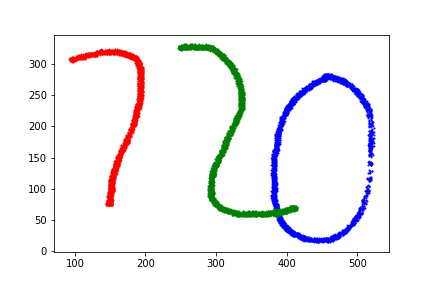
\includegraphics[width=0.37  \textwidth]{normal_720.png}
\hspace{-2em}
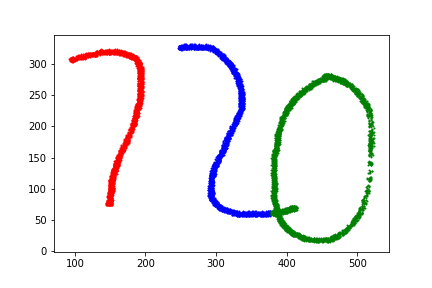
\includegraphics[width=0.37  \textwidth]{eta_large.png}
\hspace{-2em}
\vspace{-1em}
\caption{[Left]: $\eta = 0.1$,  [Middle]: $\eta = 0.5$,  [Right]: $\eta = 1.0$}
\label{fig4}
\end{figure}


\begin{figure}[htbp]
\centering
\vspace{-1em}
\hspace{-2em}
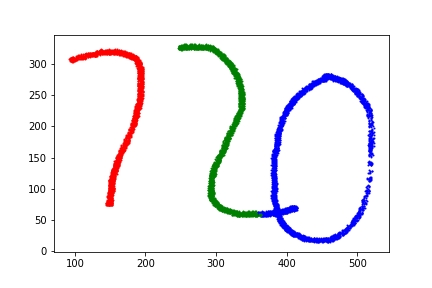
\includegraphics[width=0.37  \textwidth]{r_small.png}
\hspace{-2em}
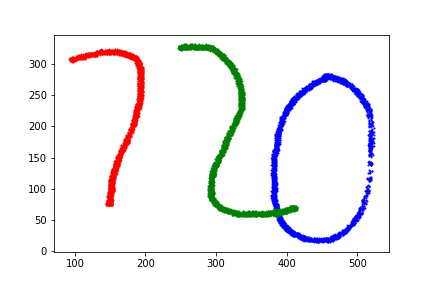
\includegraphics[width=0.37  \textwidth]{normal_720.png}
\hspace{-2em}
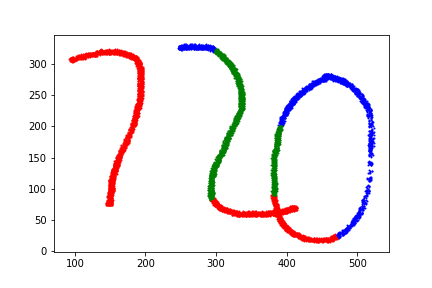
\includegraphics[width=0.37  \textwidth]{r_large.png}
\hspace{-2em}
\vspace{-1em}
\caption{[Left]: $r = 3.0$,  [Middle]: $r = 10.0$,  [Right]: $r = 40.0$}
\label{fig5}
\end{figure}
\begin{figure}[htbp]
\centering
\vspace{-1em}
\hspace{-2em}
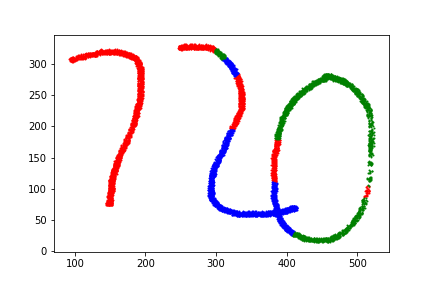
\includegraphics[width=0.37  \textwidth]{eps_small.png}
\hspace{-2em}
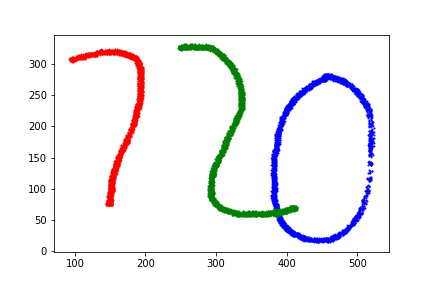
\includegraphics[width=0.37  \textwidth]{normal_720.png}
\hspace{-2em}
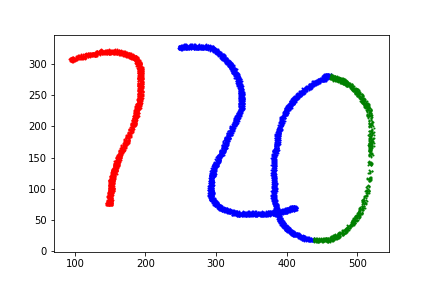
\includegraphics[width=0.37  \textwidth]{eps_large.png}
\hspace{-2em}
\vspace{-1em}
\caption{[Left]: $\epsilon = 3.0$,  [Middle]: $\epsilon = 10.0$,  [Right]: $\epsilon = 40.0$}
\label{fig6}
\end{figure}


When $\eta$ is small, local directions of data tend to have a more important role in clustering than geometric closeness between data.
In fact, in \autoref{fig4} [Left], only horizontal parts of ``7" and ``2" are labeled as green.
On the other hand, in \autoref{fig4} [Right], the orthogonal intersection doesn't work as a separating point between the vertical and the horizontal, and then a part of ``2" is absorbed in ``0".

$r$ should be chosen so that small circles with radius $r$ can appropriately cover the thickness of lines or surfaces of data points.
If $r$ is too small, the small circles may be buried in lines or surfaces.
If $r$ is too large, some circle may totally wrap around an intersection.
In both cases, the classification will fail as described in \autoref{fig5} [Left] and [Right].
\autoref{fig7} shows an enlarged view of the boundary between the blue and green areas in \autoref{fig5} [Left].
A small green circle buried in the line can be seen here.

\begin{figure}[htbp]
\centering

\includegraphics[width=0.3  \textwidth]{boundary.png}
\vspace{-1em}
\caption{Small green circle buried in the line}
\label{fig7}
\end{figure}

When $\epsilon$ is small, the affinity based on geometric distance decays immediately.
Therefore it is natural that figure \autoref{fig6} [Left] has a mottled pattern.
Conversely, when $\epsilon$ is large, the affinity remains higher over a wide distance.

%!TEX root = main.tex

\section{Application: Arithmetics autograder}
In the application of arithmetics autograder, the input image is ususally very large (typically around \(3000\times2000\) pixels), among which 10\% are black pixels.
This means if we apply ``Algorithm 4'' directly, the input list of coordinates typically have length \(10^5\) to \(10^6\), which is too long for the algorithm to return the results in reasonable period of time.
A more promising approach is to split the procedure into the following steps:
\begin{enumerate}
    \vspace{-1.0em}
    \item cluster the worksheet into equations
    \vspace{-1.0em}
    \item cluster the numbers and operators in each equation from step 1.
    \vspace{-1.0em}
    \item handwritten recognition
\end{enumerate}

\subsection{Equation clustering}
One observation is that step 1 does not need accuracy in the numbers and operators, so that we can resample the input image so that the input for Algorithm 4 is significantly reduced (to around \(10^3\) coordinates of black pixels).
\begin{figure}[htbp]
    \vspace{-1em}
    \centering
    \begin{subfigure}[t]{0.45\textwidth}
        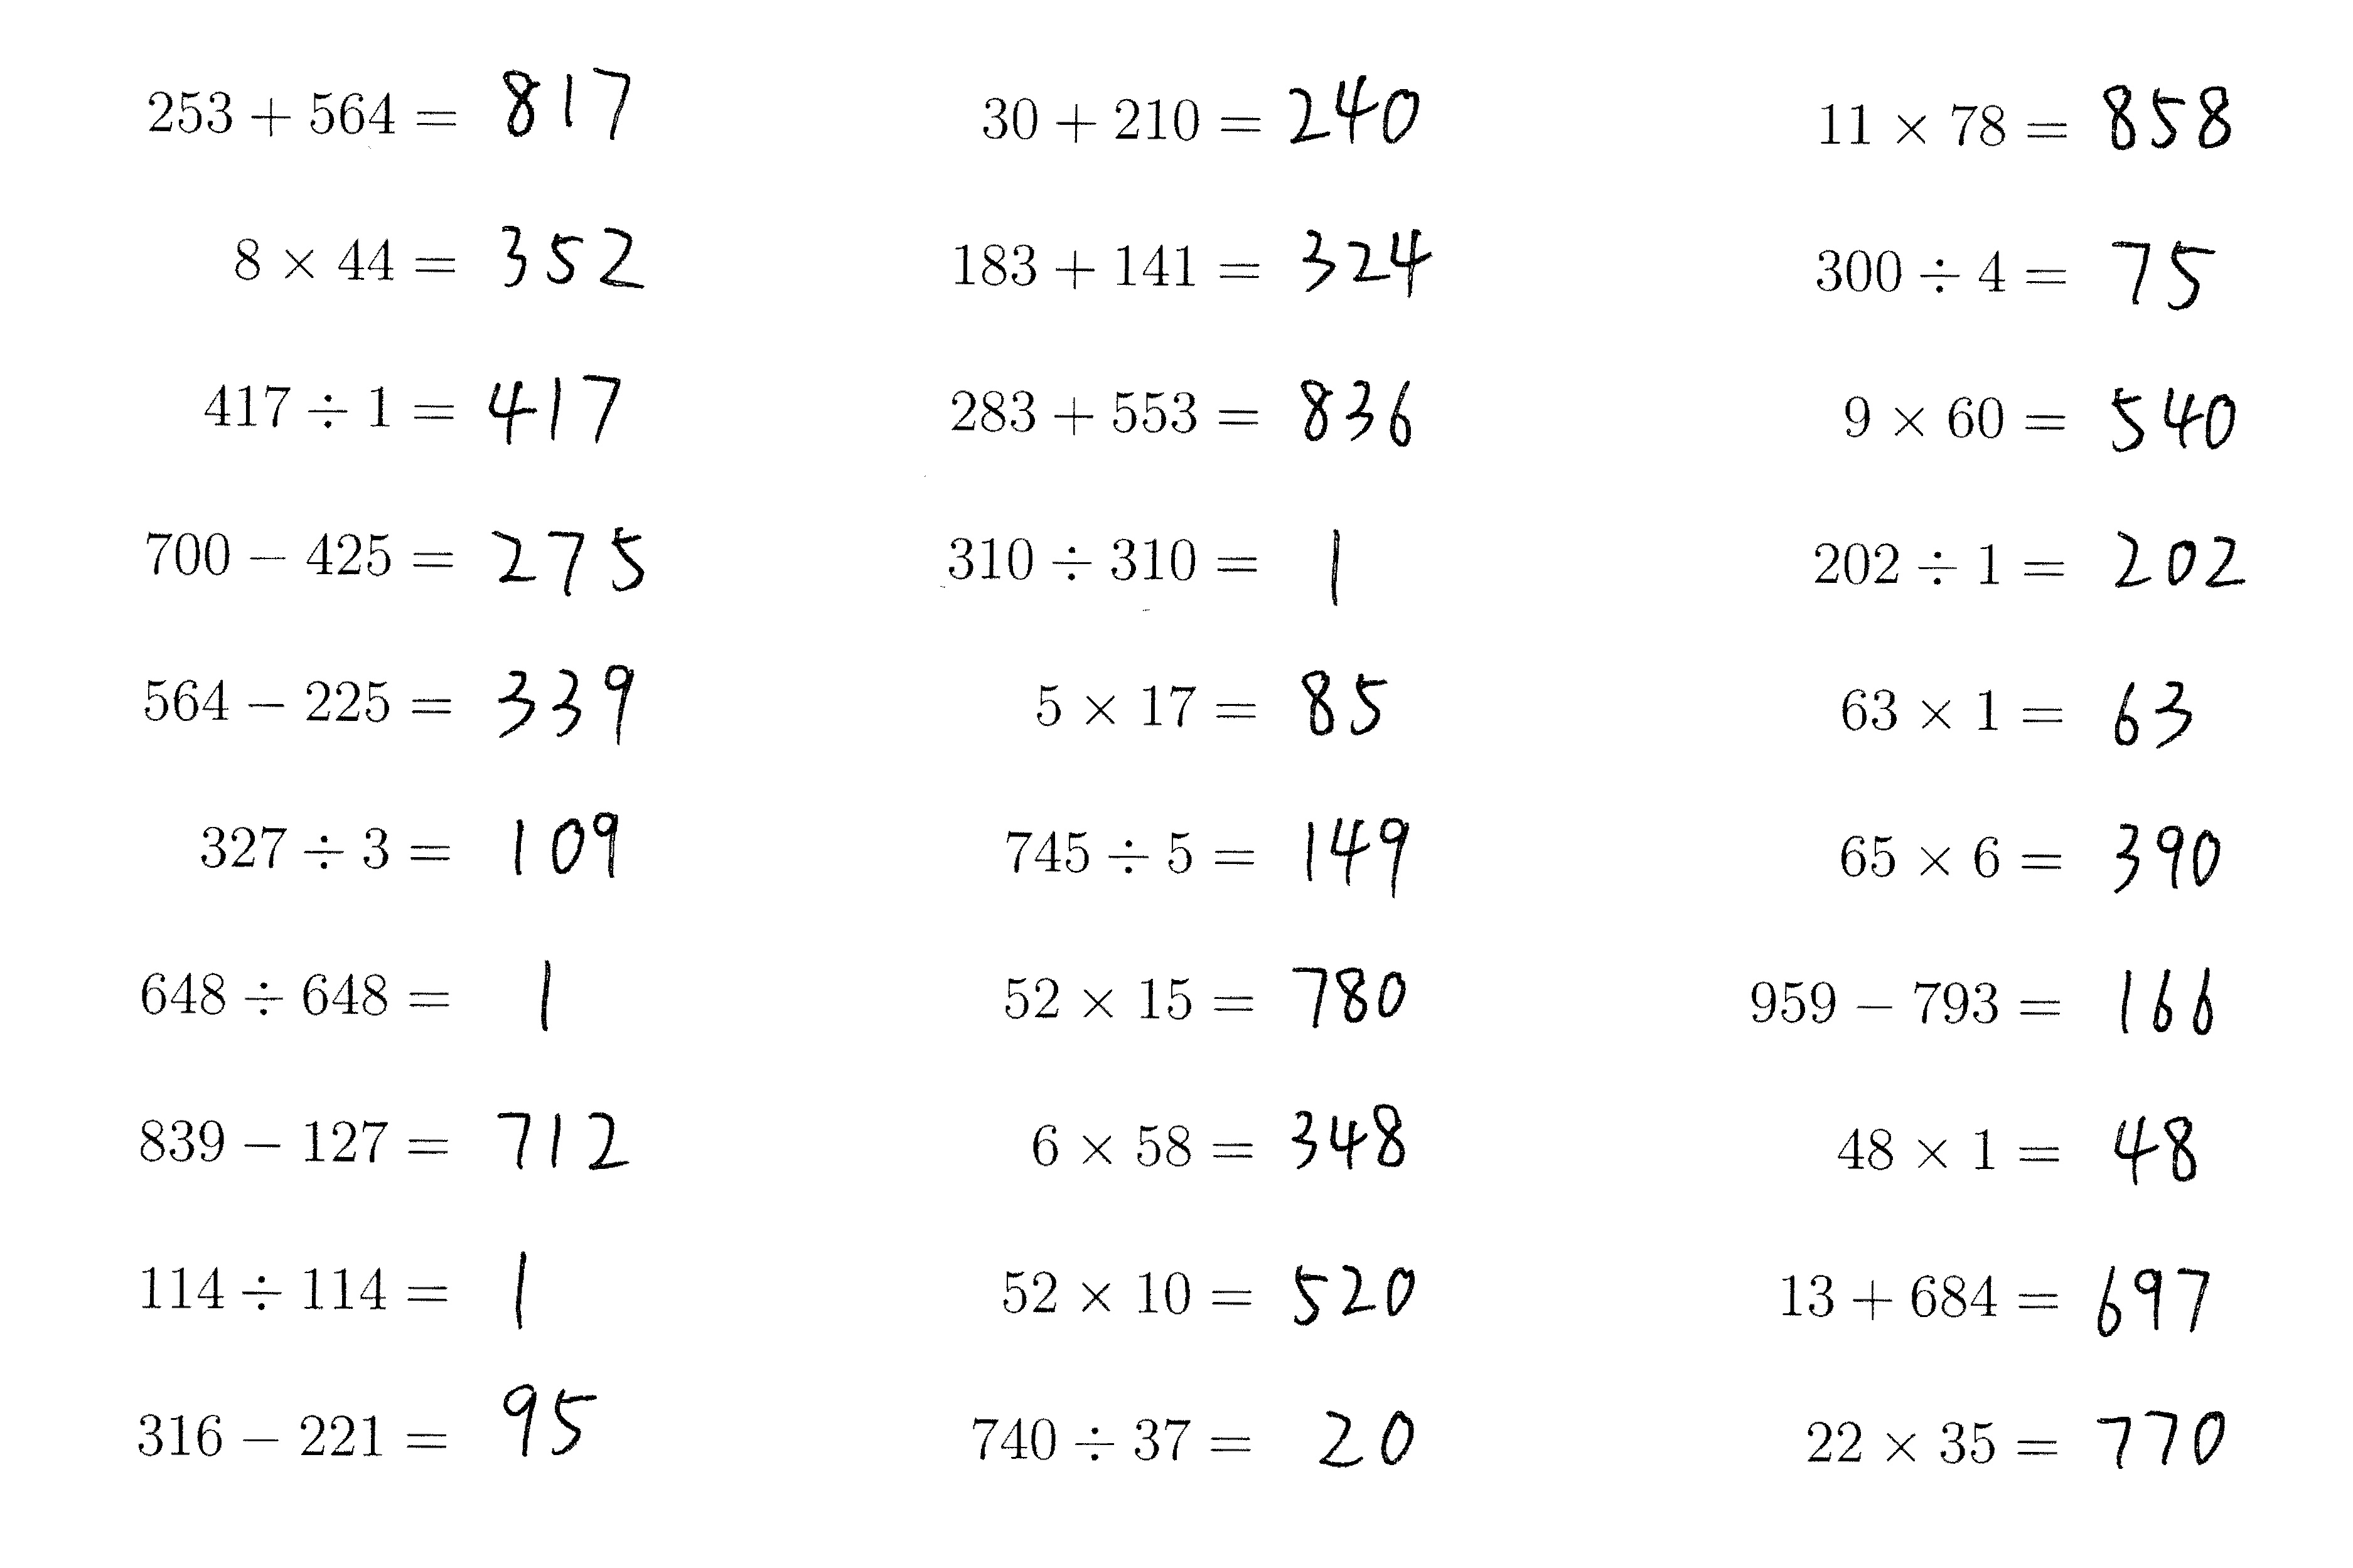
\includegraphics[width=\textwidth]{../TestSamplePictures/test1.png}
        \caption{Input image}\label{fig10a}		
    \end{subfigure}
    \begin{subfigure}[t]{0.54\textwidth}
        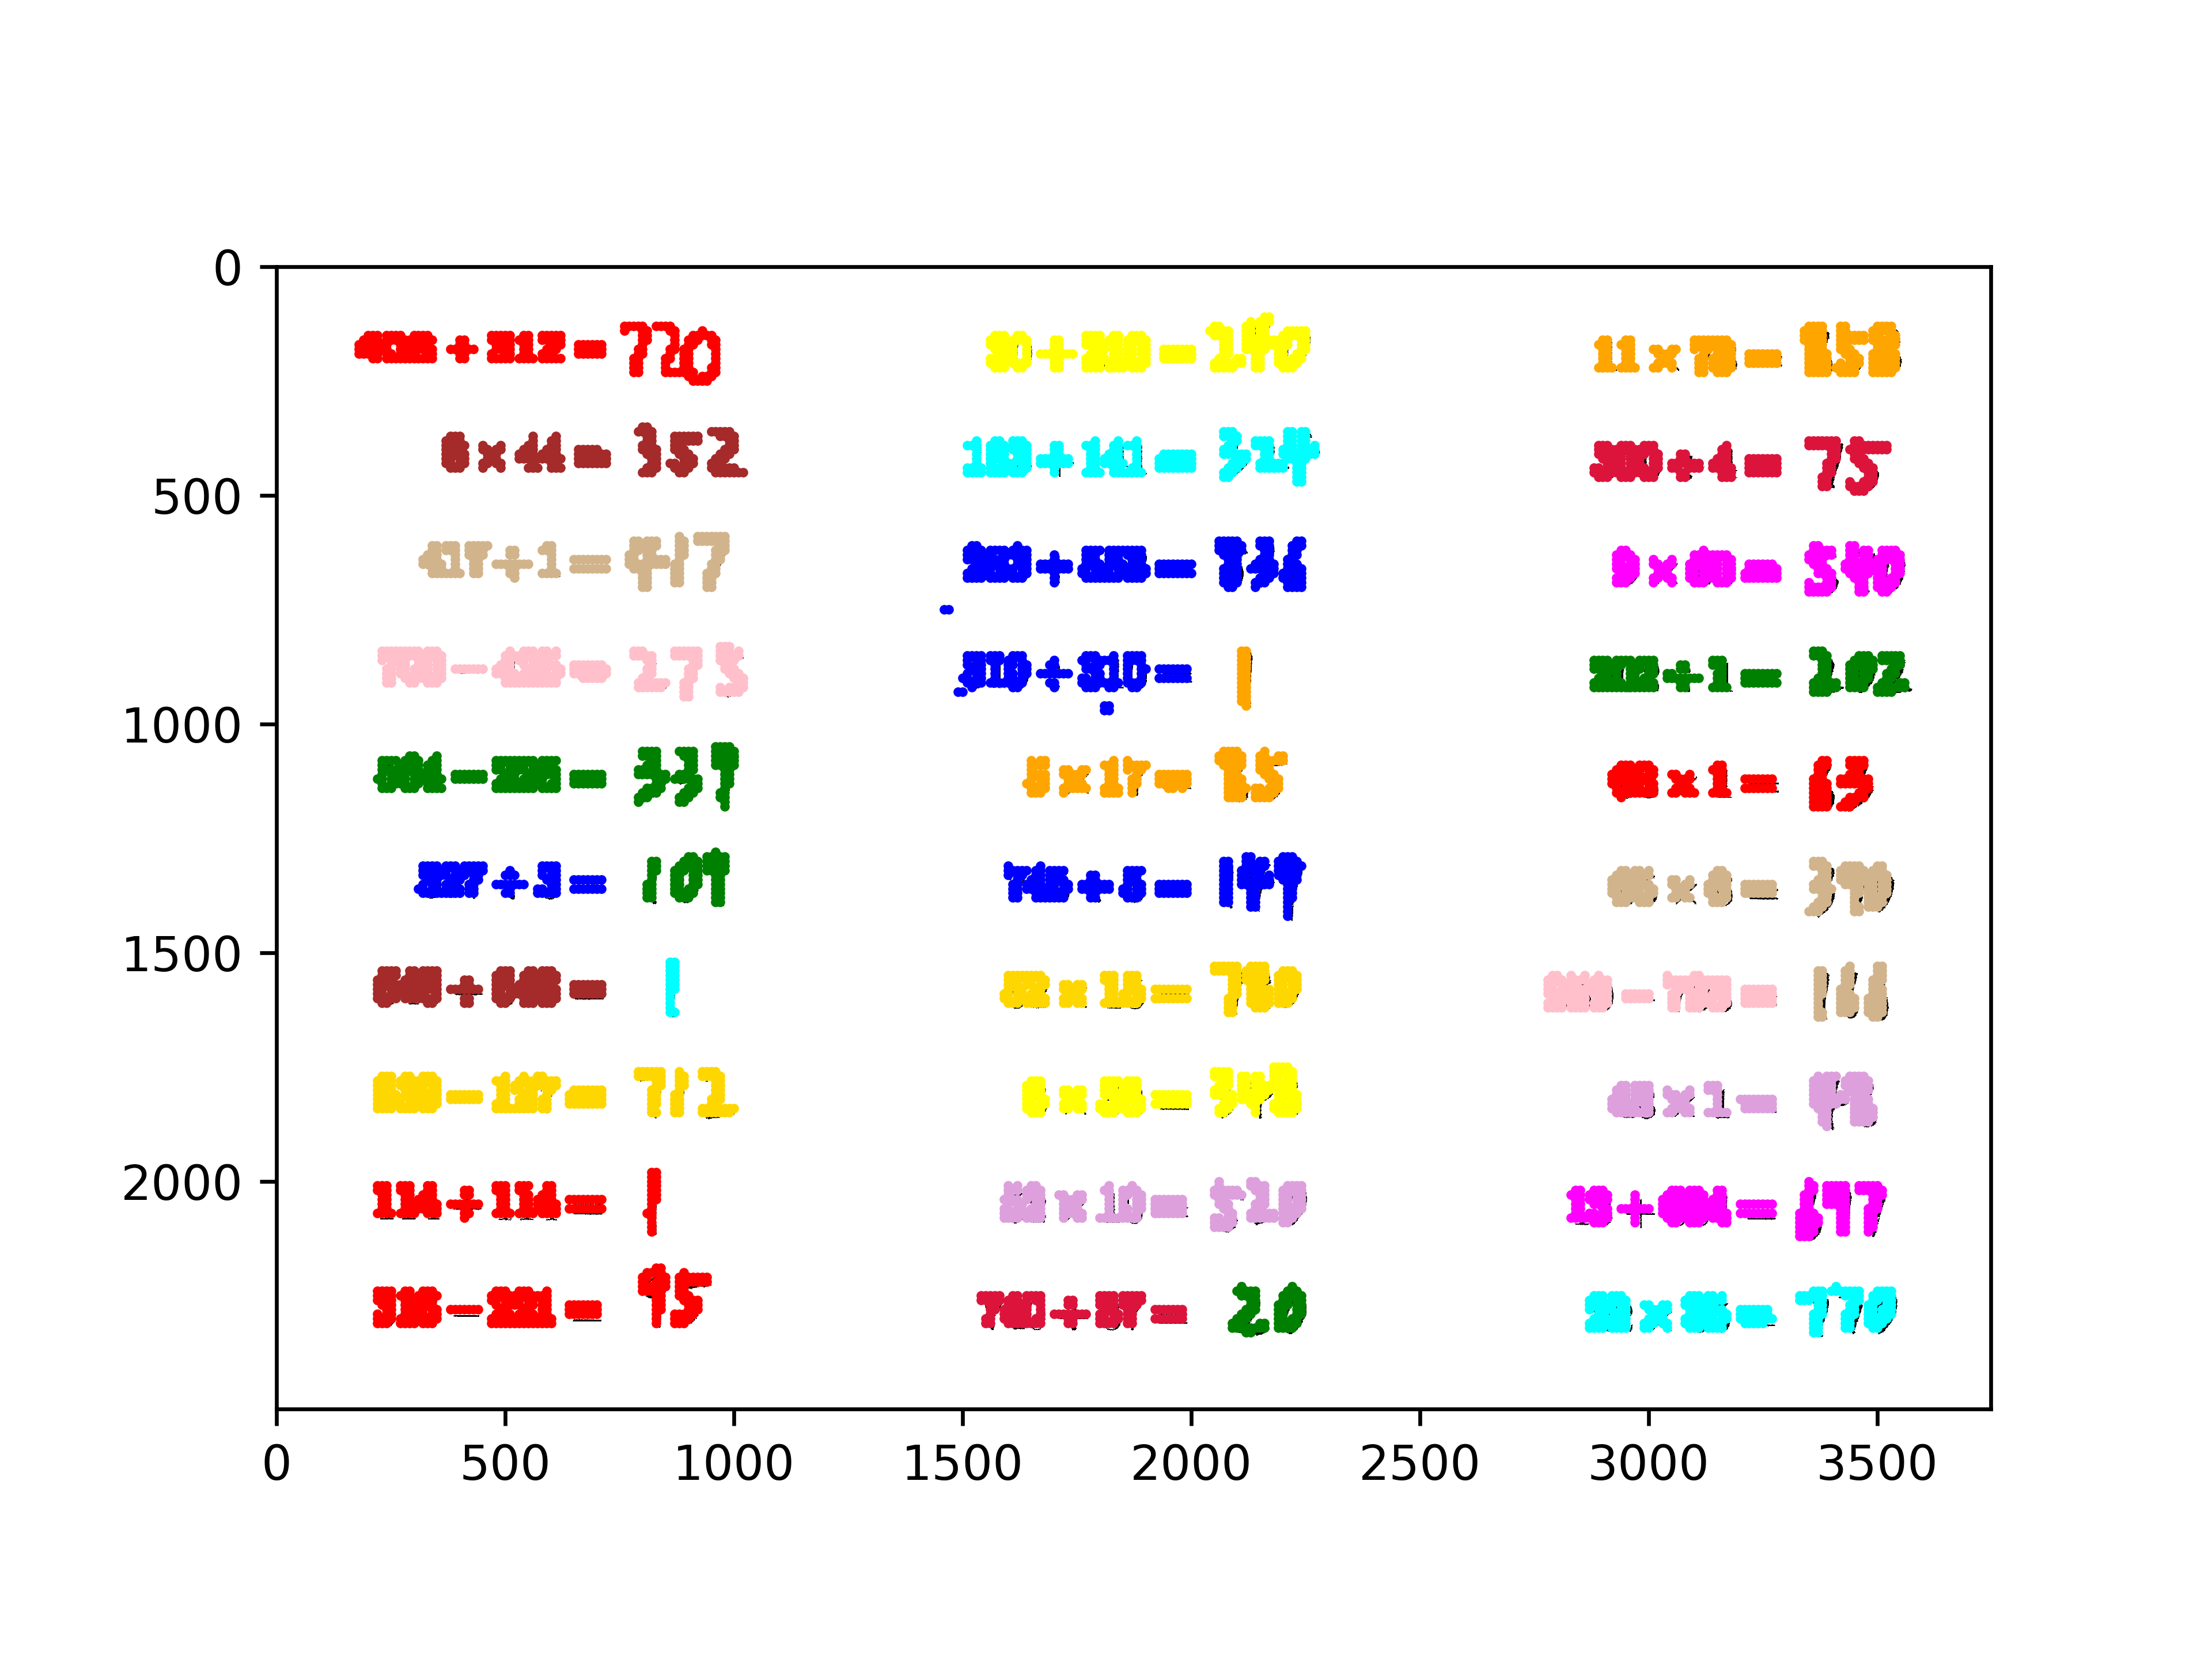
\includegraphics[width=\textwidth]{../TestSamplePictures/test_result.png}
        \caption{Equation clustering effect}\label{fig10b}
    \end{subfigure}
    \caption{Equation clustering by Algorithm 4}\label{fig10}
\end{figure}
We can see from \autoref{fig10b} is blurred compared with the input \autoref{fig10a}, and most of the equations are correctly clustered.

\subsection{Numbers and operators clustering}
We take the first equation ``408 + 312 = 720" as an example and apply Algorithm 4 again.
The main goal in this section is to divide the equation into separete digits and symbols. Especially we deal with the intersection between handwritten ``2" and handwritten ``0". See \autoref{fig10}.

\begin{figure}[htbp]
    \vspace{-1em}
    \centering
    \begin{subfigure}[t]{0.6\textwidth}
        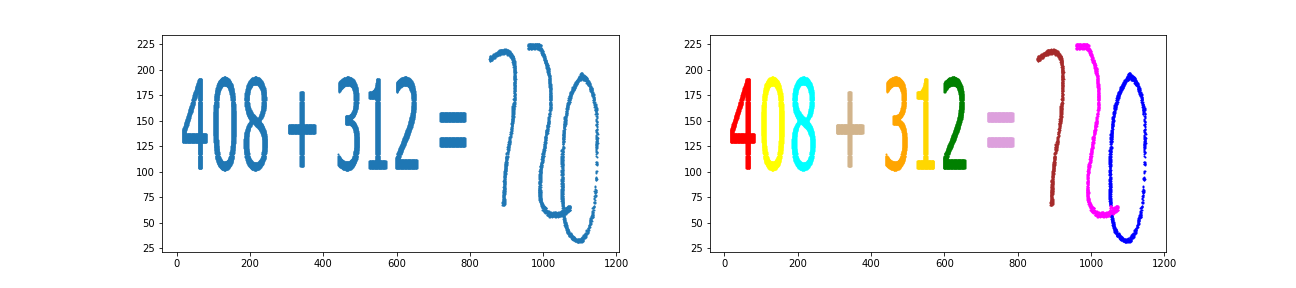
\includegraphics[width=\textwidth]{720_formula_output_1.png}
    \end{subfigure}
    \caption{Equation clustering by Algorithm 4}\label{fig10}
\end{figure}

\subsection{Handwritten recognition}
We implement handwritten recognition by using PCA. 
The results shows that we successfully recognize handwritten ``7" and ``2" but failed in handwritten ``0". 
However, it quite depends on the database we use, MNIST.
Handwritten digit recognition is a well-studied problem. Readers can use existing packages from open platform to handle this problem.
Since this is an irrelevant problem of our main project, we leave it as a future work.


\section{Conclusion}
In this project, we study new algorithms based on local PCA.
The main contribution behind this paper is that dealing with the situations where the surfaces intersect and a strong mathematical theorem guarantees the algorithms with high probability to succeed.
However, smoothness assumption is crucial to the algorithm and does not always hold in applications.
Another drawback behind the algorithm is that the points near the intersections may generate a new cluster of their own.
But it is still a competitive method in spectral clustering, and we give an application in the real world to demonstrate the ability to handle the intersections.

                

% Acknowledgements should go at the end, before appendices and references

\acks{
\textbf{Jia Guo} reads the proofs of theorems in the paper and conduct mathematical analysis on our implementation.
\textbf{Masaya Tsukamoto} write the code of the algorithm and designed some testcases, including hand-written digit generation and smooth intersecting manifolds for separation.
\textbf{Zihan Wang} writes the introduction and additional algorithm in the paper we study.
\textbf{Guangting Yu} implements the arithmetic autograding based on the algorithm and compare with other existing algorithms.
Every group member writes the report together and contributes to the project equally.
}

% Manual newpage inserted to improve layout of sample file - not
% needed in general before appendices/bibliography.

\newpage

\appendix

\vskip 0.2in
% \bibliography{sample}
% \bibliographystyle{apalike}
\bibliography{ml}
\end{document}